\glsresetall
\chapter{Methodology}
\label{chap:methodology}

The methodology of work carried out in this research project is presented in this chapter. First, every member involved will be mentioned as well as their individual contribution for the project. Second, the adopted approach and process organisation of the collaborators involved will be explained. Finally, the work plan as well as the work performed, including the foreseen and real work plans for the whole year of work are presented.

The main people involved in this project were myself, André Pascoal Bento, student at the Master course of Informatics Engineering at \gls{dei}, who carried out the investigation and development of the project. In second, Prof. Filipe Araújo, assistant professor at the University of Coimbra, who contributed with his vast knowledge and guidance on topics about distributed systems and cloud computing. In third, Prof. Jorge Cardoso, Chief Architect for Intelligent CloudOps at Huawei Technologies, who contributed with his vision, great contact with the topics addressed in this work and with the tracing data set from Huawei Cloud Platform~\cite{huawei_cloud_platform}. In fourth, Eng. Jaime Correia, doctoral student at \gls{dei}, who contributed with his vast technical knowledge regarding the topics of tracing and monitoring microservices.

\todo{CONTINUE FROM HERE!!!}

As this work stands for an investigation, it was necessary to perform an exploratory work and there were no clear development methodology adopted. Instead of a development methodology, meetings were scheduled in the beginning to happen every two weeks. In this meetings, the people mentioned in the previous paragraph were gathered together to discuss the work carried out in the last two weeks and topics like the information gathered, the analysis about some existing tools, ideas and solutions were discussed between all. In the end, although there wasn't defined some development methodology, the meeting that were carried out were more than enough to keep the productivity and good work.

For the work plan and starting by some numbers, the time spent in each semester of the year by week are sixteen hours for the first semester, and forty hours for the second one. In the end, it was spent a total of 304 hours for the first semester, starting in 11.09.2018 and ending in 21.01.2019 (19 weeks times 16 hours per week), and it is expected to be spent a total of 840 hours for the second semester, starting in 04.02.2019 and ending in 30.06.2019 (21 weeks times 40 hours per week).

In the beginning, there was a work plan for two semesters given in the project proposition. For record, these plans are presented in Figure~\ref{fig:proposed_work_plan_semester_1_and_2}.

For effects of analysis, the real work plan carried out in the first semester is presented in Figure~\ref{fig:real_work_plan_semester_1}.

\begin{figure}[H]
    \centering
    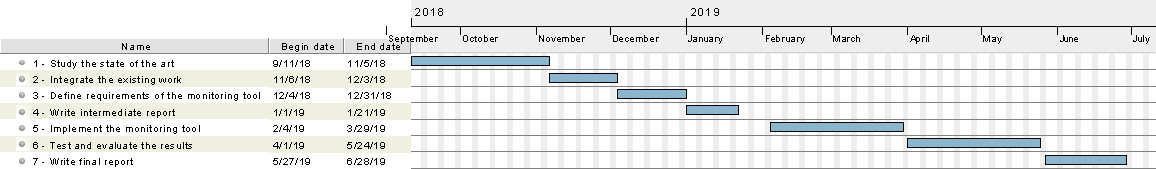
\includegraphics[width=1.00\textwidth]{images/proposed_work_plan_semester_1_and_2.pdf}
    \caption{Proposed work plan for the first and second semesters.}
    \label{fig:proposed_work_plan_semester_1_and_2}
\end{figure}

\begin{figure}[H]
    \centering
    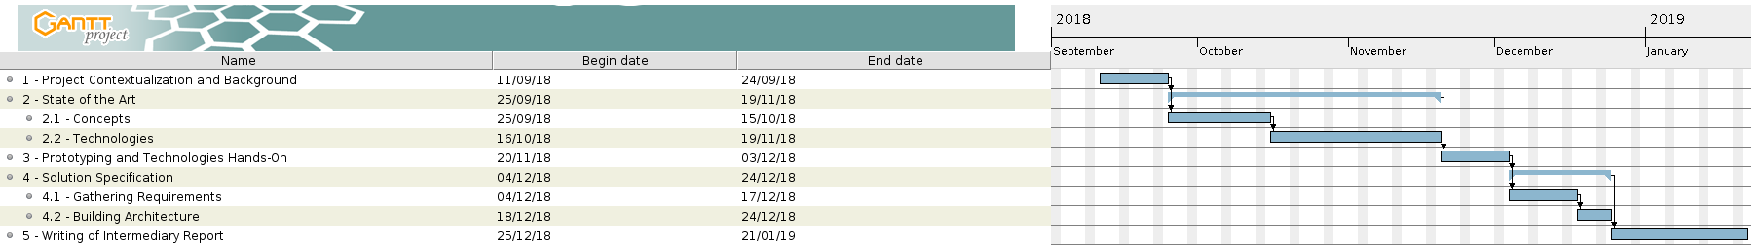
\includegraphics[width=1.00\textwidth, height=0.25\textwidth]{images/real_work_plan_semester_1.pdf}
    \caption{Real work plan for the first semester.}
    \label{fig:real_work_plan_semester_1}
\end{figure}

As we can see, the ``foreseen'' work plan for the first semester has suffered some changes, when comparing it to the real work plan. The predicted task 1 - Study the state of the art(...), was branched into two 1 - Project Contextualisation and Background and 2 - State of the Art, and took some more time to do because of the non-concrete and lack of documentation in the technologies related to the subject of this thesis. The predicted task 2 - Integrate the existing work, was replaced by 3 - Prototyping and Technologies Hands-On. This replacement was done because of the interest in test the technologies gathered in the state of the art and see some results with them, enhancing our investigation work and allowing us to get a better visualisation of the data that we had back then. The remaining tasks took almost the predicted time to do.

Finally, it was generated a foreseen work plan for the second semester even knowing that, with almost one hundred percent of certainty the work plan will change when we perform the real work, it is presented in the figure \ref{fig:foreseen_work_plan_semester_2}. This work plan was generated taken into account the proposed work presented in the figure \ref{fig:proposed_work_plan_semester_2} and the effort needed to implement the defined solution presented in the chapter \ref{chap:possible_solution} - \nameref{chap:possible_solution}. To estimate the effort for each task we decided to, first group tasks by four groups regarding their complexity and work load, second discuss if they were in the right group taking into consideration what is defined in the solution and the task background knowledge, and third assign the defined values to each group. This values represent the work days for each task, and in this case we defined the following four: 3(three), 5(five), 8(eight) and 12(twelve) working days as they are akin to the Fibonacci suites\cite{project_estimation_times}. The only task that were not submitted to this, was the task 3 - Write the final report.

\begin{figure}[H]
    \centering
    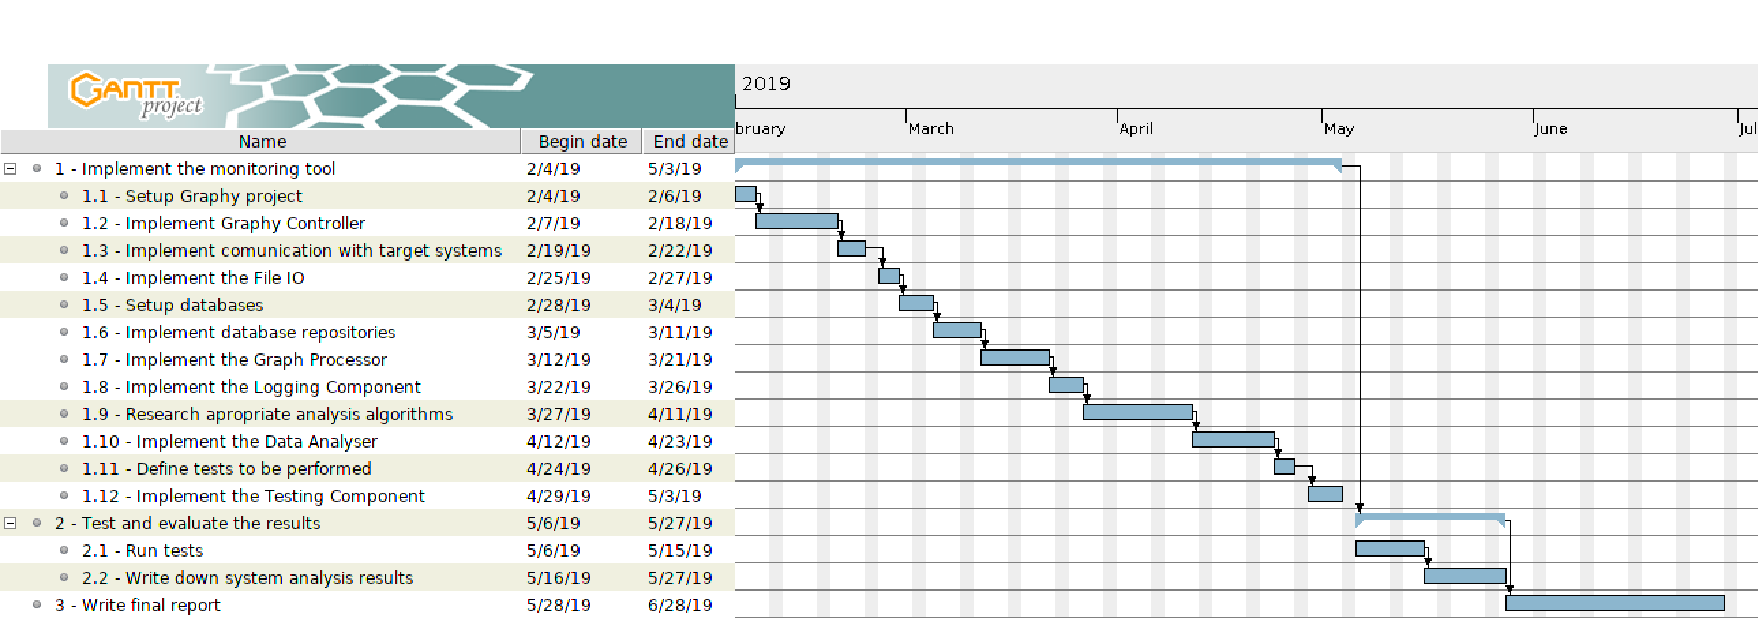
\includegraphics[width=1.00\textwidth]{images/foreseen_work_plan_semester_2.pdf}
    \caption{Foreseen work plan for the second semester.}
    \label{fig:foreseen_work_plan_semester_2}
\end{figure}

\begin{figure}[H]
    \centering
    %\includegraphics[width=1.00\textwidth]{images/real_work_plan_semester_2.pdf}
    \caption{Real work plan for the second semester.}
    \label{fig:real_work_plan_semester_2}
\end{figure}

All the figures to expose the work plans have been created by an open-source tool called GanttProject\cite{gantt_project_tool} that produce Gantt charts, a kind of diagram used to illustrate the progress of the different stages of a project.

%-------------------------------------------------------------------------------------------------
\checkoddpage
\ifthenelse{\boolean{oddpage}}
{ % Odd page
\newpage
\blankpage}
{ % Even page
}
%-------------------------------------------------------------------------------------------------